% This file was created with tikzplotlib v0.9.17.
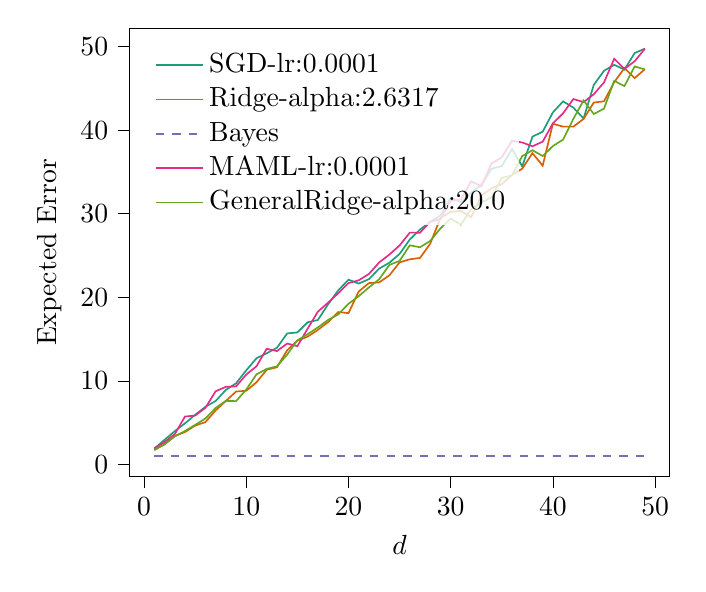
\begin{tikzpicture}

\definecolor{color0}{rgb}{0.105882352941176,0.619607843137255,0.466666666666667}
\definecolor{color1}{rgb}{0.850980392156863,0.372549019607843,0.00784313725490196}
\definecolor{color2}{rgb}{0.458823529411765,0.43921568627451,0.701960784313725}
\definecolor{color3}{rgb}{0.905882352941176,0.16078431372549,0.541176470588235}
\definecolor{color4}{rgb}{0.4,0.650980392156863,0.117647058823529}

\begin{axis}[
legend cell align={left},
legend style={
  fill opacity=0.8,
  draw opacity=1,
  text opacity=1,
  at={(0.03,0.97)},
  anchor=north west,
  draw=none
},
tick align=outside,
tick pos=left,
x grid style={white!69.0196078431373!black},
xlabel={\(\displaystyle d\)},
xmin=-1.4, xmax=51.4,
xtick style={color=black},
y grid style={white!69.0196078431373!black},
ylabel={Expected Error},
ymin=-1.43764292359485, ymax=52.1859445711913,
ytick style={color=black}
]
\addplot [semithick, color0]
table {%
1 1.90454225916568
2 2.9526403351813
3 3.99074469923969
4 4.92542809599303
5 5.94827206579716
6 6.89979111651147
7 7.59802203130015
8 8.92641239498088
9 9.71589192554616
10 11.2716134246486
11 12.7088311795247
12 13.310257940246
13 13.9640761102041
14 15.6818612233912
15 15.7987206491015
16 17.0139904877685
17 17.2855018569967
18 19.1519885939313
19 20.838308991673
20 22.1093532260448
21 21.6441252879155
22 22.1719468636379
23 23.4348052468121
24 24.1392340221816
25 25.18862976769
26 26.9149125039429
27 28.1123376477121
28 29.0092461749645
29 29.8027970955389
30 31.9226699605627
31 31.3725362447514
32 32.5026932531404
33 33.4588446313533
34 35.3764689785918
35 35.7011090762749
36 37.7488436609692
37 35.6613897236057
38 39.2175798889808
39 39.810238510152
40 42.1206552293384
41 43.4418585458056
42 42.6875612907659
43 41.3919003564996
44 45.4056856144632
45 47.0947526206968
46 47.8043740649546
47 47.2408050688137
48 49.2142352465236
49 49.7485087759738
};
\addlegendentry{SGD-lr:0.0001}
\addplot [semithick, color1]
table {%
1 1.72412857881576
2 2.42125949750688
3 3.4100356535189
4 3.88419320719546
5 4.65975689893652
6 5.06872167351103
7 6.47387114185241
8 7.60104262298374
9 8.73081352050767
10 8.82251940894168
11 9.84202567835748
12 11.3369379014968
13 11.6317962897328
14 13.6711844969781
15 14.8148606949547
16 15.2934422342278
17 16.1019035762553
18 17.0301208421161
19 18.2357034490621
20 18.1094913610415
21 20.7013987415443
22 21.7009043267375
23 21.7823409006246
24 22.6268727158795
25 24.1796373120055
26 24.5478473997086
27 24.7115421719401
28 26.4198273196089
29 29.4906788022487
30 30.219566745838
31 30.3360389522218
32 29.5853816164781
33 32.1619408387968
34 33.0370757912447
35 33.5369538644329
36 34.6493407812418
37 35.3824271658983
38 37.2423770813883
39 35.7456277535183
40 40.7634068153725
41 40.4141108559395
42 40.4117682445975
43 41.3346308278218
44 43.2981122191369
45 43.4426387172639
46 45.7350704797478
47 47.4201560452508
48 46.2190502047281
49 47.2917805646145
};
\addlegendentry{Ridge-alpha:2.6317}
\addplot [semithick, color2, dashed]
table {%
1 0.9997928716227
2 0.9997928716227
3 0.9997928716227
4 0.9997928716227
5 0.9997928716227
6 0.9997928716227
7 0.9997928716227
8 0.9997928716227
9 0.9997928716227
10 0.9997928716227
11 0.9997928716227
12 0.9997928716227
13 0.9997928716227
14 0.9997928716227
15 0.9997928716227
16 0.9997928716227
17 0.9997928716227
18 0.9997928716227
19 0.9997928716227
20 0.9997928716227
21 0.9997928716227
22 0.9997928716227
23 0.9997928716227
24 0.9997928716227
25 0.9997928716227
26 0.9997928716227
27 0.9997928716227
28 0.9997928716227
29 0.9997928716227
30 0.9997928716227
31 0.9997928716227
32 0.9997928716227
33 0.9997928716227
34 0.9997928716227
35 0.9997928716227
36 0.9997928716227
37 0.9997928716227
38 0.9997928716227
39 0.9997928716227
40 0.9997928716227
41 0.9997928716227
42 0.9997928716227
43 0.9997928716227
44 0.9997928716227
45 0.9997928716227
46 0.9997928716227
47 0.9997928716227
48 0.9997928716227
49 0.9997928716227
};
\addlegendentry{Bayes}
\addplot [semithick, color3]
table {%
1 1.91508997378672
2 2.68827625899063
3 3.63229127100003
4 5.73826466341989
5 5.85955809200194
6 6.78196745641214
7 8.75557713345996
8 9.29792177397122
9 9.34898687400509
10 10.7609858504507
11 11.7539072081211
12 13.8500728065156
13 13.5678700553635
14 14.4697615355164
15 14.160631222951
16 16.2434569675654
17 18.281384797889
18 19.3517713090439
19 20.4883662292192
20 21.708470831287
21 22.0318768054882
22 22.7939567070857
23 24.174690175679
24 25.1126566309533
25 26.2029151915037
26 27.7358691950036
27 27.7287980535447
28 29.061819683904
29 29.3501844578414
30 31.5244590937878
31 31.6878271815177
32 33.8819249285483
33 33.2733679599489
34 36.0025287129306
35 36.7440760529333
36 38.7338344777112
37 38.5191911893039
38 38.0627182117804
39 38.6172771708639
40 40.8089602390849
41 42.0113363534537
42 43.7179543338979
43 43.3488731423426
44 44.284989253422
45 45.7047791638564
46 48.5375857305713
47 47.315840271559
48 48.238713792507
49 49.731120925676
};
\addlegendentry{MAML-lr:0.0001}
\addplot [semithick, color4]
table {%
1 1.76755964192367
2 2.40477233570909
3 3.36511495788206
4 4.00487748620587
5 4.74317462502509
6 5.50499605692064
7 6.76199088515107
8 7.60925970501405
9 7.58369565539883
10 8.97270866241096
11 10.7828652729641
12 11.4375889225807
13 11.7436235238865
14 13.1483697358577
15 14.8571605646999
16 15.5918603602446
17 16.3996849554053
18 17.2916355855251
19 17.9617523276285
20 19.2258003886668
21 20.1354358786715
22 21.1856070051504
23 22.1564819791886
24 23.8703589401048
25 24.3606602659324
26 26.2188042393067
27 25.9868398576163
28 26.7438650514298
29 28.2490097460973
30 29.4176883135791
31 28.6951277227144
32 30.5257222309795
33 31.3432472931864
34 31.9741328134877
35 34.2868132151525
36 34.5831378838334
37 36.8949134199437
38 37.5963967423638
39 36.8966289798475
40 38.0930926803809
41 38.8632482752151
42 41.3385271722031
43 43.5547244563212
44 41.9223560829734
45 42.5722773584946
46 45.8896603707724
47 45.2624496069521
48 47.6175138968456
49 47.2552132820741
};
\addlegendentry{GeneralRidge-alpha:20.0}
\end{axis}

\end{tikzpicture}
